
\begin{figure}[H]
  {
    \setlength{\tabcolsep}{3.0pt}
    \setlength\cmidrulewidth{\heavyrulewidth} % Make cmidrule = 
    \begin{adjustbox}{width=3cm,center}
      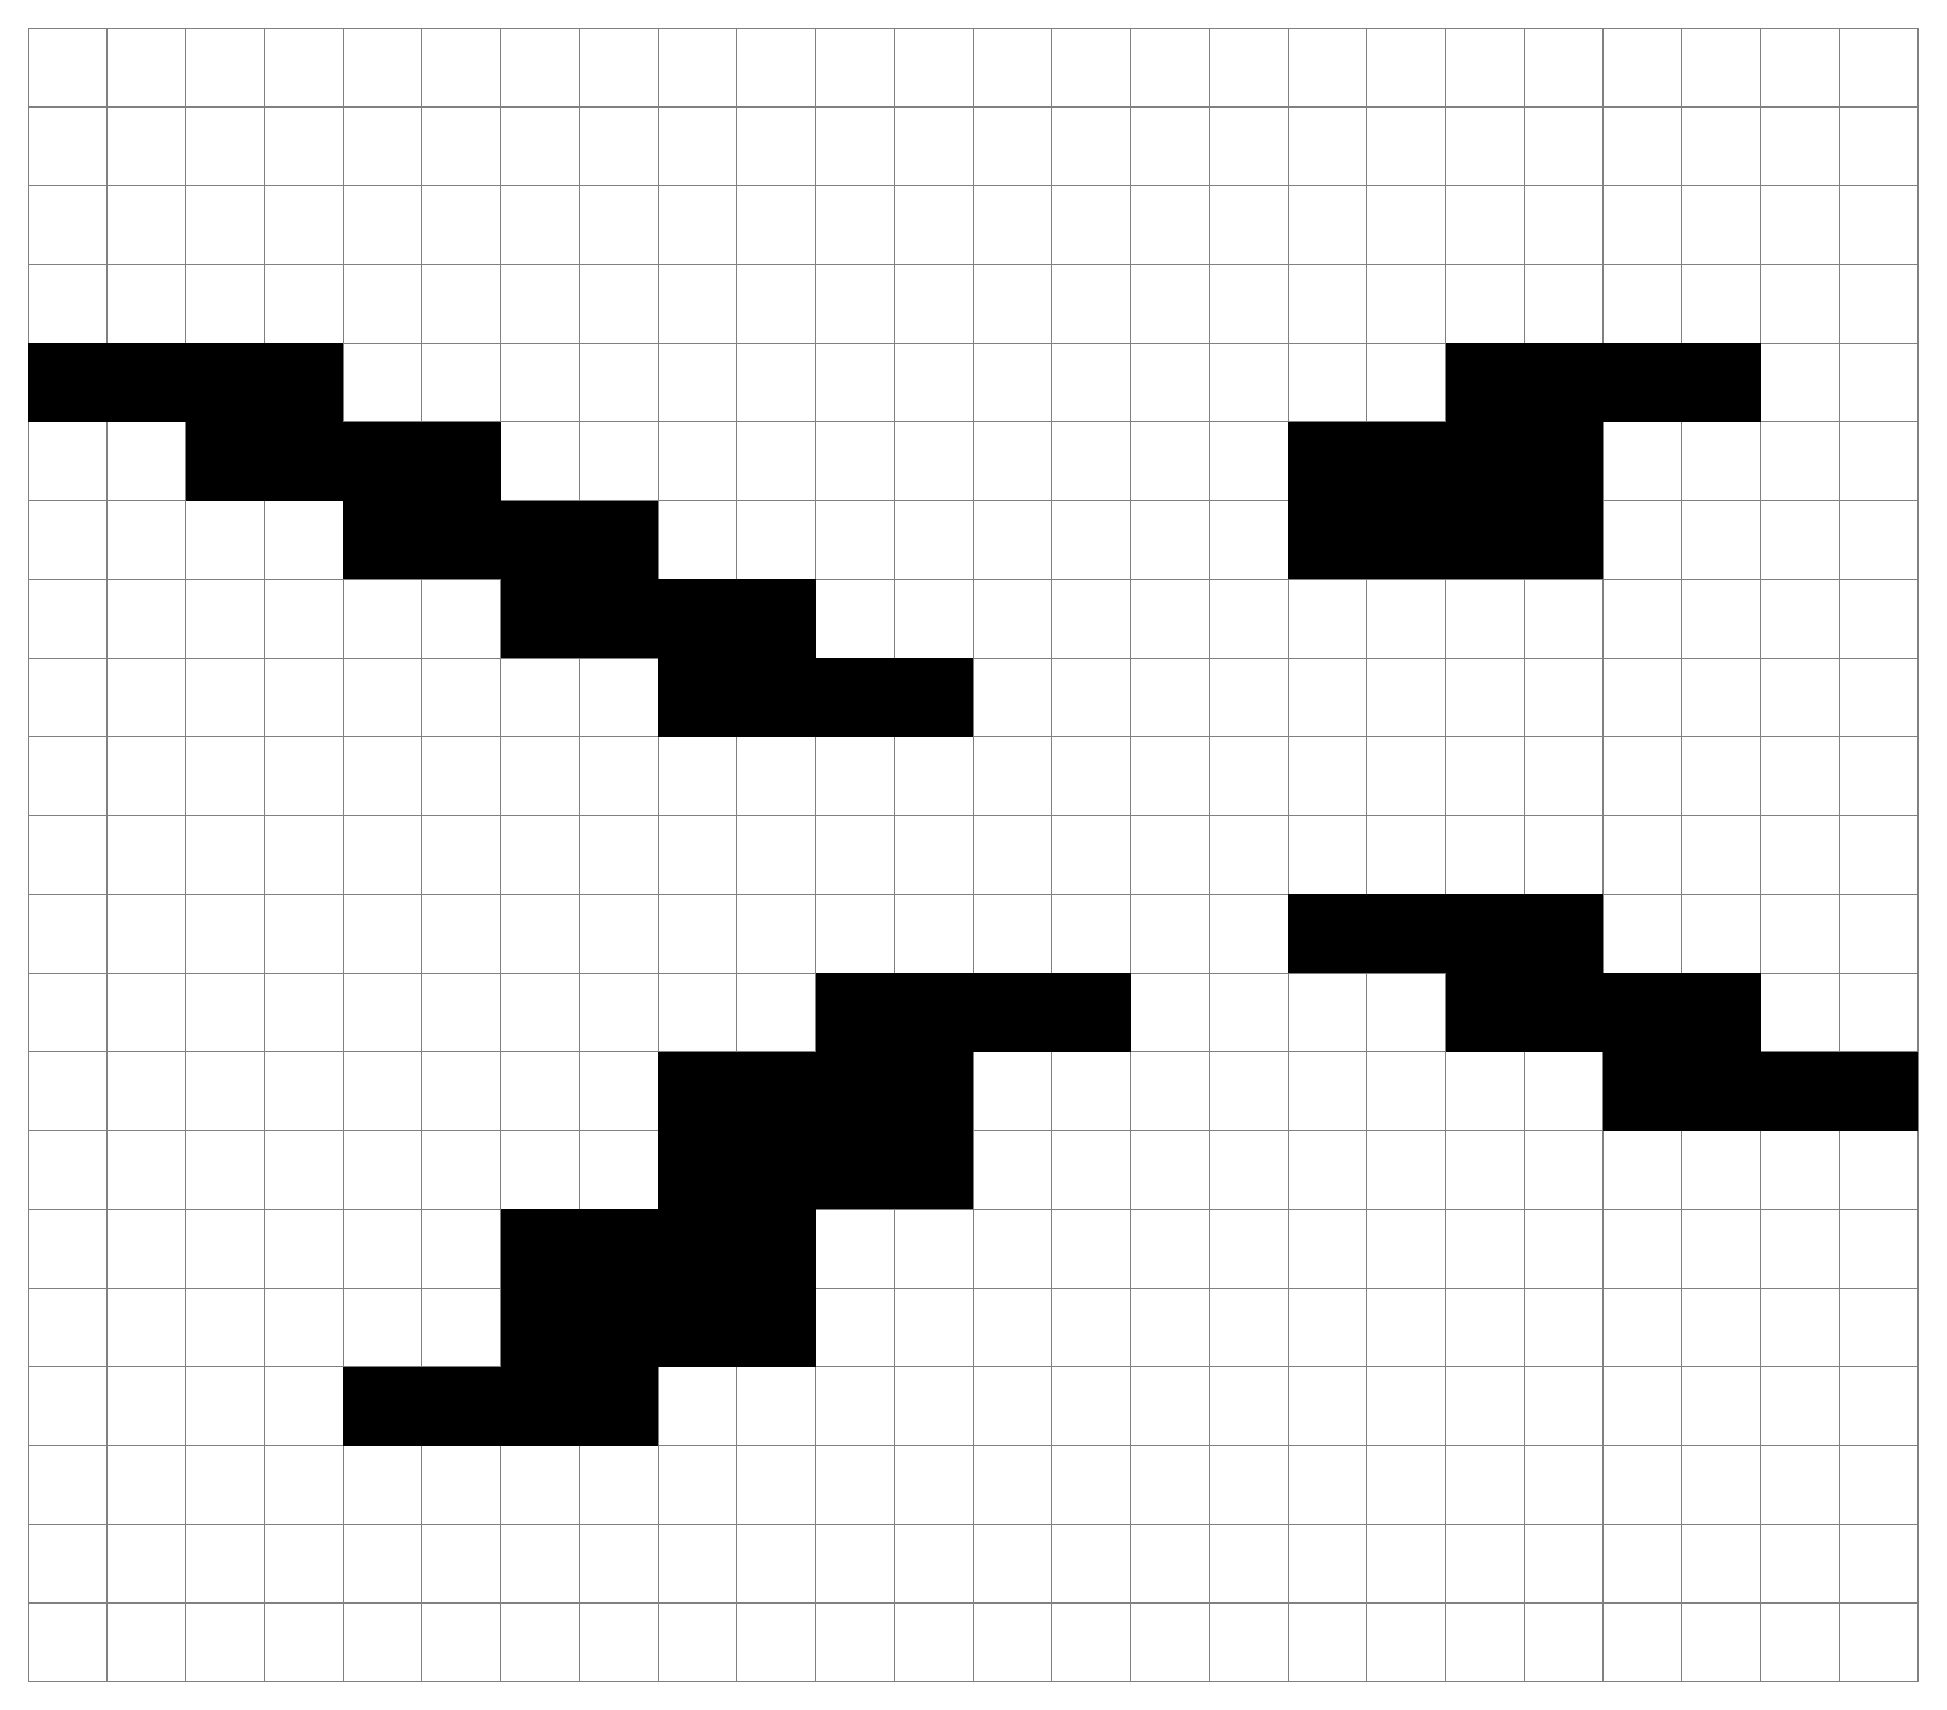
\begin{tikzpicture}

	\draw[step=1.0,gray,thin] (0,0) grid (24,21);
	\fill[\SPRITECOLOR] (0,16) rectangle ++ (1,1);
	\fill[\SPRITECOLOR] (1,16) rectangle ++ (1,1);
	\fill[\SPRITECOLOR] (2,16) rectangle ++ (1,1);
	\fill[\SPRITECOLOR] (3,16) rectangle ++ (1,1);
	\fill[\SPRITECOLOR] (18,16) rectangle ++ (1,1);
	\fill[\SPRITECOLOR] (19,16) rectangle ++ (1,1);
	\fill[\SPRITECOLOR] (20,16) rectangle ++ (1,1);
	\fill[\SPRITECOLOR] (21,16) rectangle ++ (1,1);
	\fill[\SPRITECOLOR] (2,15) rectangle ++ (1,1);
	\fill[\SPRITECOLOR] (3,15) rectangle ++ (1,1);
	\fill[\SPRITECOLOR] (4,15) rectangle ++ (1,1);
	\fill[\SPRITECOLOR] (5,15) rectangle ++ (1,1);
	\fill[\MULTICOLORONE] (16,15) rectangle ++ (1,1);
	\fill[\MULTICOLORONE] (17,15) rectangle ++ (1,1);
	\fill[\MULTICOLORONE] (18,15) rectangle ++ (1,1);
	\fill[\MULTICOLORONE] (19,15) rectangle ++ (1,1);
	\fill[\MULTICOLORONE] (4,14) rectangle ++ (1,1);
	\fill[\MULTICOLORONE] (5,14) rectangle ++ (1,1);
	\fill[\MULTICOLORONE] (6,14) rectangle ++ (1,1);
	\fill[\MULTICOLORONE] (7,14) rectangle ++ (1,1);
	\fill[\MULTICOLORONE] (16,14) rectangle ++ (1,1);
	\fill[\MULTICOLORONE] (17,14) rectangle ++ (1,1);
	\fill[\MULTICOLORONE] (18,14) rectangle ++ (1,1);
	\fill[\MULTICOLORONE] (19,14) rectangle ++ (1,1);
	\fill[\MULTICOLORONE] (6,13) rectangle ++ (1,1);
	\fill[\MULTICOLORONE] (7,13) rectangle ++ (1,1);
	\fill[\MULTICOLORONE] (8,13) rectangle ++ (1,1);
	\fill[\MULTICOLORONE] (9,13) rectangle ++ (1,1);
	\fill[\MULTICOLORONE] (8,12) rectangle ++ (1,1);
	\fill[\MULTICOLORONE] (9,12) rectangle ++ (1,1);
	\fill[\MULTICOLORONE] (10,12) rectangle ++ (1,1);
	\fill[\MULTICOLORONE] (11,12) rectangle ++ (1,1);
	\fill[\MULTICOLORONE] (16,9) rectangle ++ (1,1);
	\fill[\MULTICOLORONE] (17,9) rectangle ++ (1,1);
	\fill[\MULTICOLORONE] (18,9) rectangle ++ (1,1);
	\fill[\MULTICOLORONE] (19,9) rectangle ++ (1,1);
	\fill[\MULTICOLORONE] (10,8) rectangle ++ (1,1);
	\fill[\MULTICOLORONE] (11,8) rectangle ++ (1,1);
	\fill[\MULTICOLORONE] (12,8) rectangle ++ (1,1);
	\fill[\MULTICOLORONE] (13,8) rectangle ++ (1,1);
	\fill[\MULTICOLORONE] (18,8) rectangle ++ (1,1);
	\fill[\MULTICOLORONE] (19,8) rectangle ++ (1,1);
	\fill[\MULTICOLORONE] (20,8) rectangle ++ (1,1);
	\fill[\MULTICOLORONE] (21,8) rectangle ++ (1,1);
	\fill[\MULTICOLORONE] (8,7) rectangle ++ (1,1);
	\fill[\MULTICOLORONE] (9,7) rectangle ++ (1,1);
	\fill[\MULTICOLORONE] (10,7) rectangle ++ (1,1);
	\fill[\MULTICOLORONE] (11,7) rectangle ++ (1,1);
	\fill[\SPRITECOLOR] (20,7) rectangle ++ (1,1);
	\fill[\SPRITECOLOR] (21,7) rectangle ++ (1,1);
	\fill[\SPRITECOLOR] (22,7) rectangle ++ (1,1);
	\fill[\SPRITECOLOR] (23,7) rectangle ++ (1,1);
	\fill[\MULTICOLORONE] (8,6) rectangle ++ (1,1);
	\fill[\MULTICOLORONE] (9,6) rectangle ++ (1,1);
	\fill[\MULTICOLORONE] (10,6) rectangle ++ (1,1);
	\fill[\MULTICOLORONE] (11,6) rectangle ++ (1,1);
	\fill[\MULTICOLORONE] (6,5) rectangle ++ (1,1);
	\fill[\MULTICOLORONE] (7,5) rectangle ++ (1,1);
	\fill[\MULTICOLORONE] (8,5) rectangle ++ (1,1);
	\fill[\MULTICOLORONE] (9,5) rectangle ++ (1,1);
	\fill[\SPRITECOLOR] (6,4) rectangle ++ (1,1);
	\fill[\SPRITECOLOR] (7,4) rectangle ++ (1,1);
	\fill[\SPRITECOLOR] (8,4) rectangle ++ (1,1);
	\fill[\SPRITECOLOR] (9,4) rectangle ++ (1,1);
	\fill[\SPRITECOLOR] (4,3) rectangle ++ (1,1);
	\fill[\SPRITECOLOR] (5,3) rectangle ++ (1,1);
	\fill[\SPRITECOLOR] (6,3) rectangle ++ (1,1);
	\fill[\SPRITECOLOR] (7,3) rectangle ++ (1,1);

      \end{tikzpicture}
    \end{adjustbox}
  }\caption{EXPLOSION\_MIDDLE}
\end{figure}
